\documentclass[12pt]{article}
  \usepackage{geometry}
 \usepackage[round]{natbib}
 \usepackage{graphicx}
 \geometry{a4paper}
  \usepackage[T1]{fontenc}
  \usepackage[utf8]{inputenc}
  \usepackage{authblk}
  \usepackage[running]{lineno}
  \usepackage{setspace}
  \usepackage{booktabs}
  \usepackage{tabularx}
  \usepackage{chngpage}
  \usepackage{amsmath}
  \usepackage{amssymb}
  \usepackage[hidelinks]{hyperref}
 \usepackage[textsize=tiny]{todonotes}


\usepackage{natbib} %package for bibliography

%   \doublespacing
% \raggedright
\title{A Meta-analysis of Longevity Estimates of Mosquito Vectors of Disease: Figures}
\author{Ben Lambert, Ace North, Charles Godfray}

\begin{document}
\maketitle

\begin{figure}[h]
	\centerline{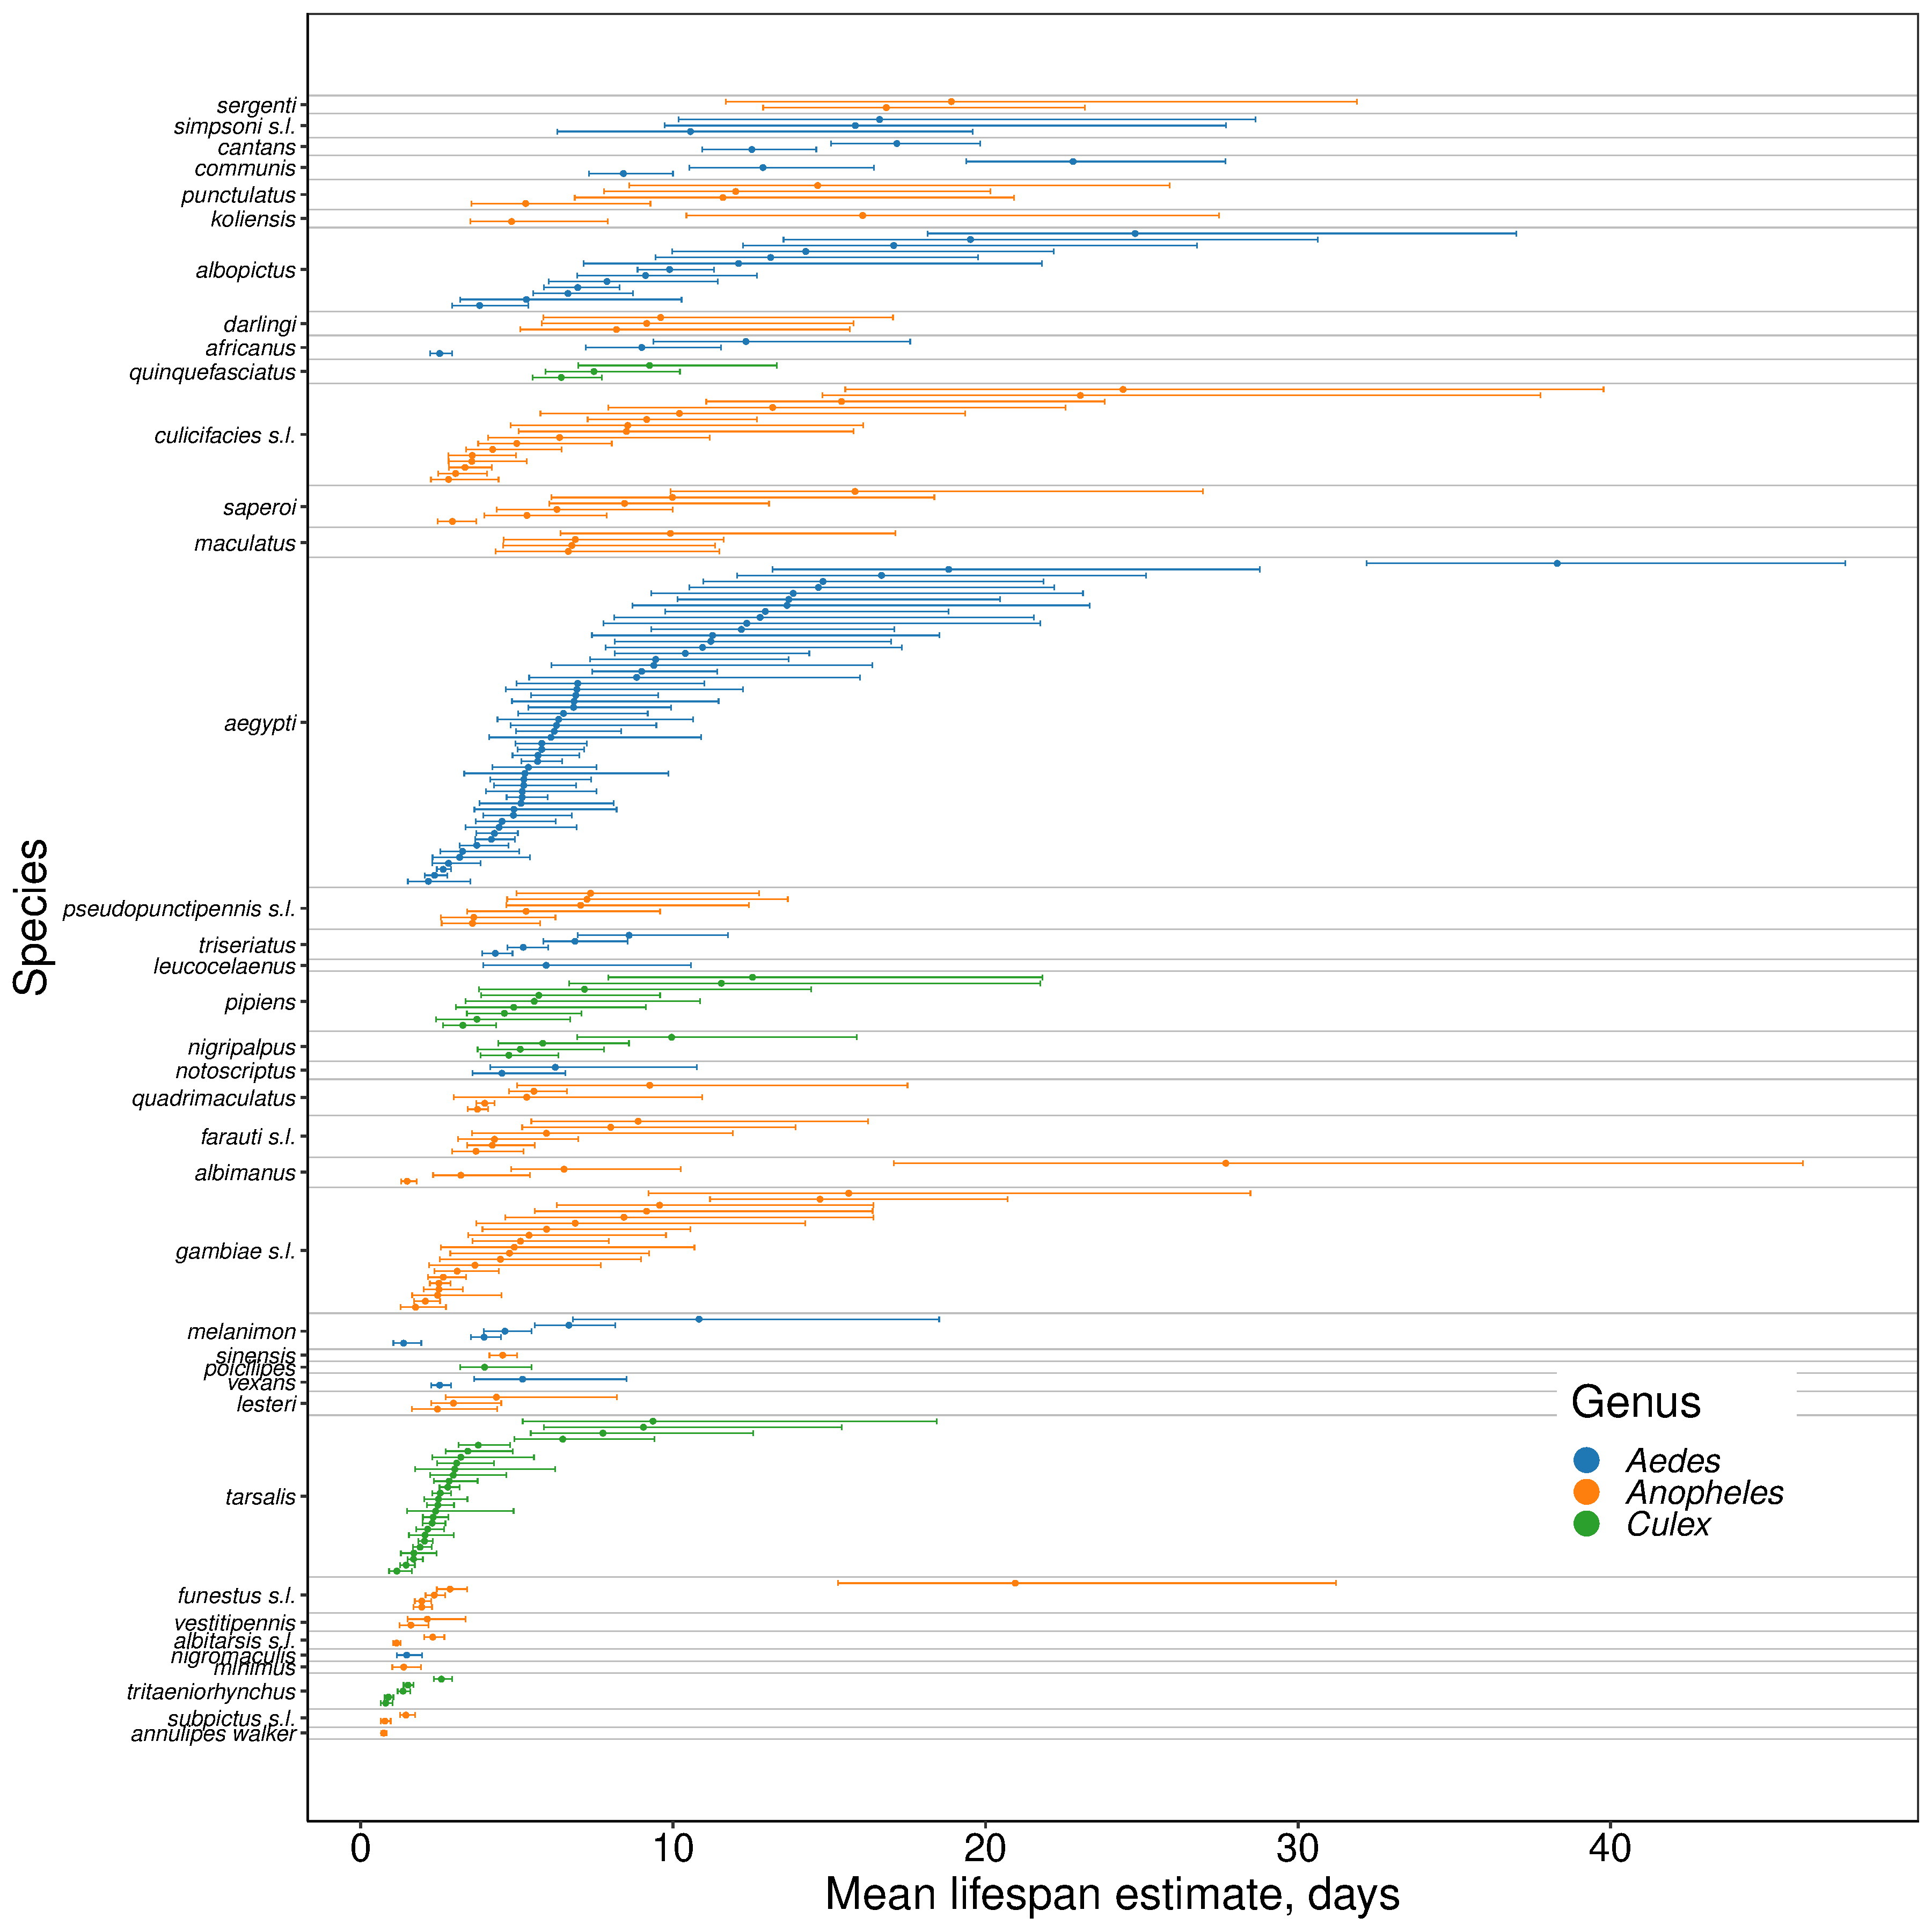
\includegraphics[width=1\textwidth]{./Figure_files/mrr_individualEstimates_allSpecies_withoutBalabacensis.pdf}}
	\caption{\textbf{MRR: lifespan estimates for each time series.} The middle point shows the median estimates, and the left and right box whiskers show the 25\%, and 75\% posterior quantiles respectively. All estimates were obtained using the non-hierarchical exponential survival model as described in text.}
	\label{fig:mrr_lifespan_individualEstimates}
\end{figure}

\begin{figure}[h]
	\centerline{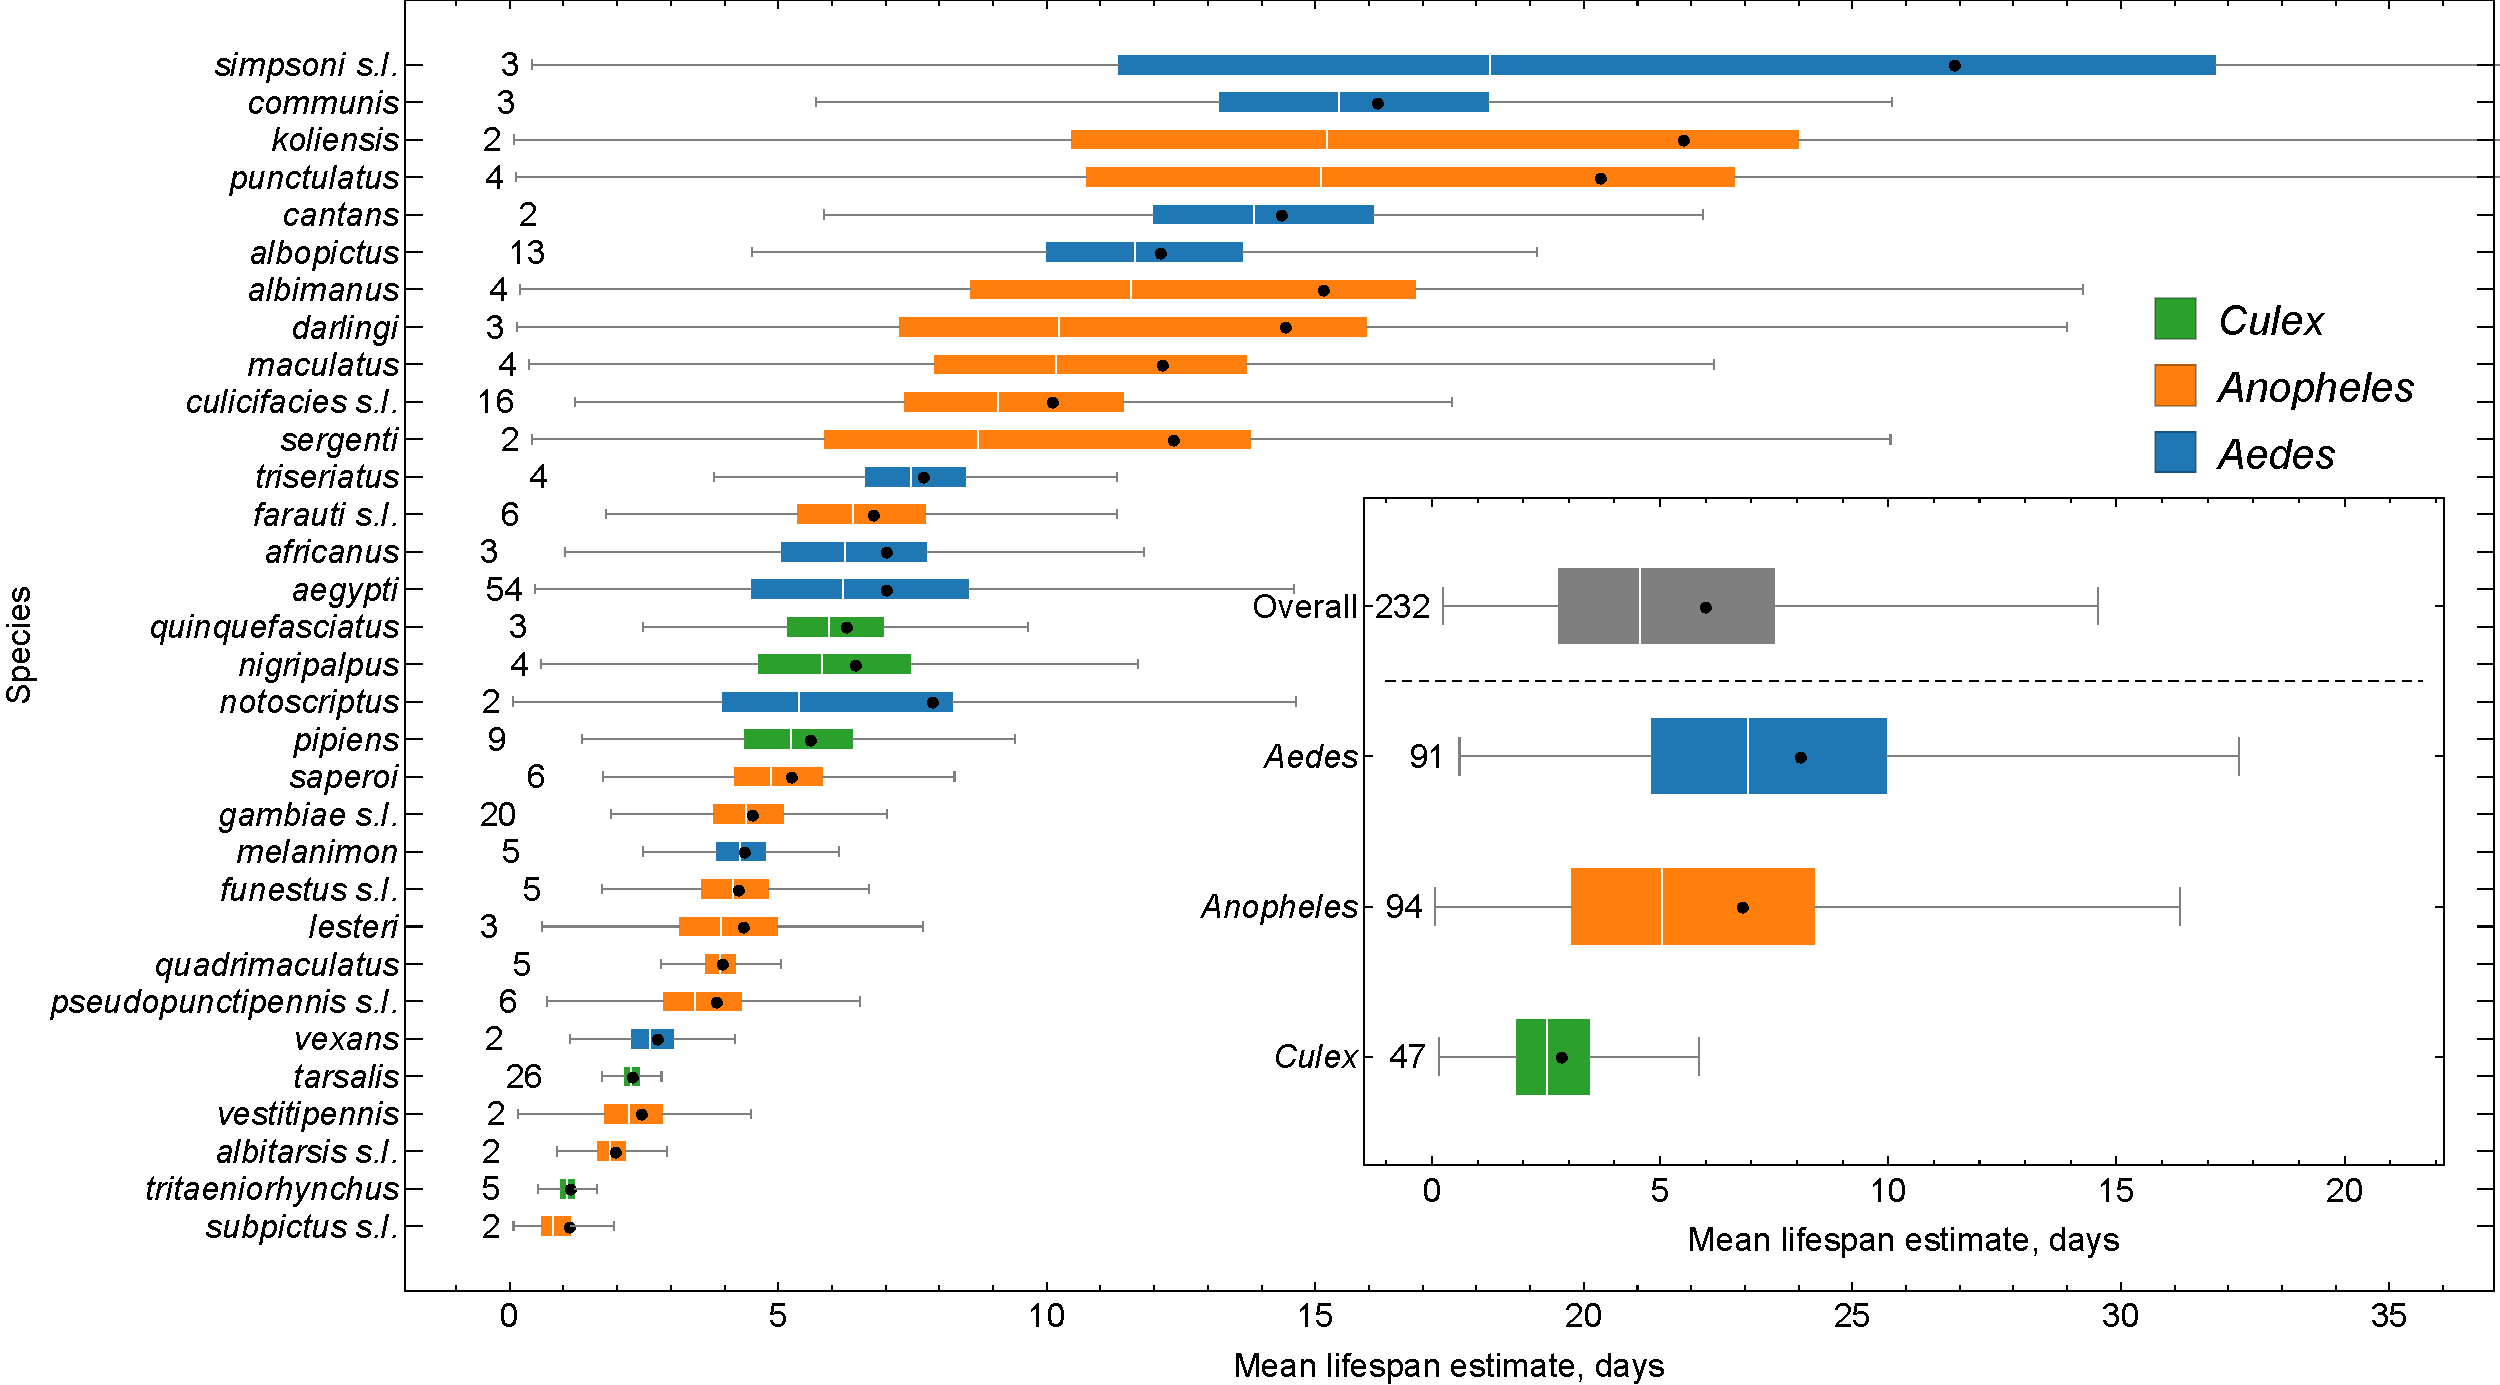
\includegraphics[width=1\textwidth]{./Figure_files/mrr_lifetimes_final_female_without_sugar_not_blood.pdf}}
	\caption{\textbf{MRR: grouped lifespan estimates.} The lifespans shown are for mosquitoes that were not fed with sugar or blood before release. The middle line in each box shows the median estimates and the solid dot indicates the mean. The left and right box edges show the 25\%, and 75\% posterior quantiles respectively. The whiskers show the range of the data, excluding points lying more than 1.5 times the interquartile range away from each edge of the box. The numbers before the start of the left whisker indicate the number of individual time-series within each species. All estimates were obtained using the hierarchical exponential survival model.}
	\label{fig:mrr_lifespans}
\end{figure}

\begin{figure}[h]
	\centerline{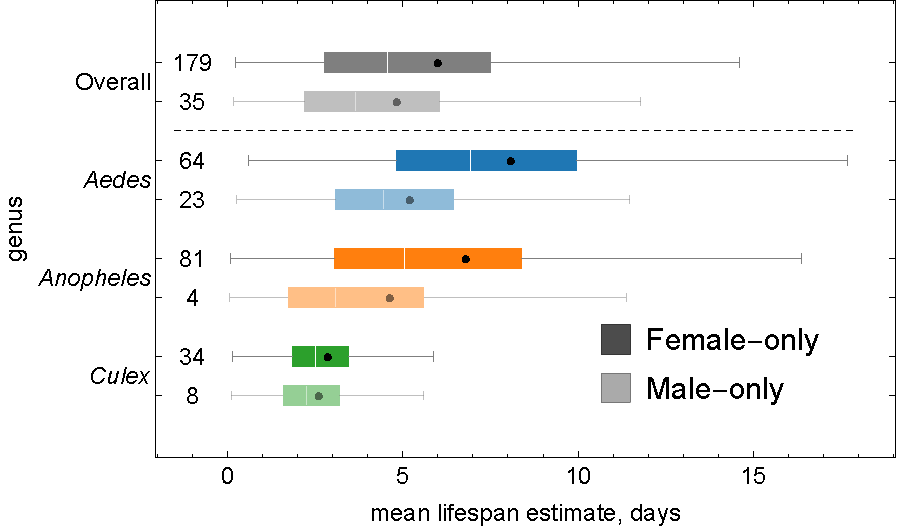
\includegraphics[width=1\textwidth]{./Figure_files/mrr_sexDifferences_without_sugar_nor_blood.pdf}}
	\caption{\textbf{MRR: lifespan estimates by sex.} The lifespans shown are for mosquitoes that were not fed with sugar or blood (for females) before release. The middle line in each box shows the median estimates and the solid dot indicates the mean. The left and right box edges show the 25\%, and 75\% posterior quantiles respectively. The whiskers show the range of the data, excluding points lying more than 1.5 times the interquartile range away from each edge of the box. The numbers before the start of the left whisker indicate the number of individual time-series within each species. All estimates were obtained using the hierarchical exponential survival model.}
	\label{fig:mrr_sexDifferences_without_sugar_nor_blood}
\end{figure}

\begin{figure}[h]
	\centerline{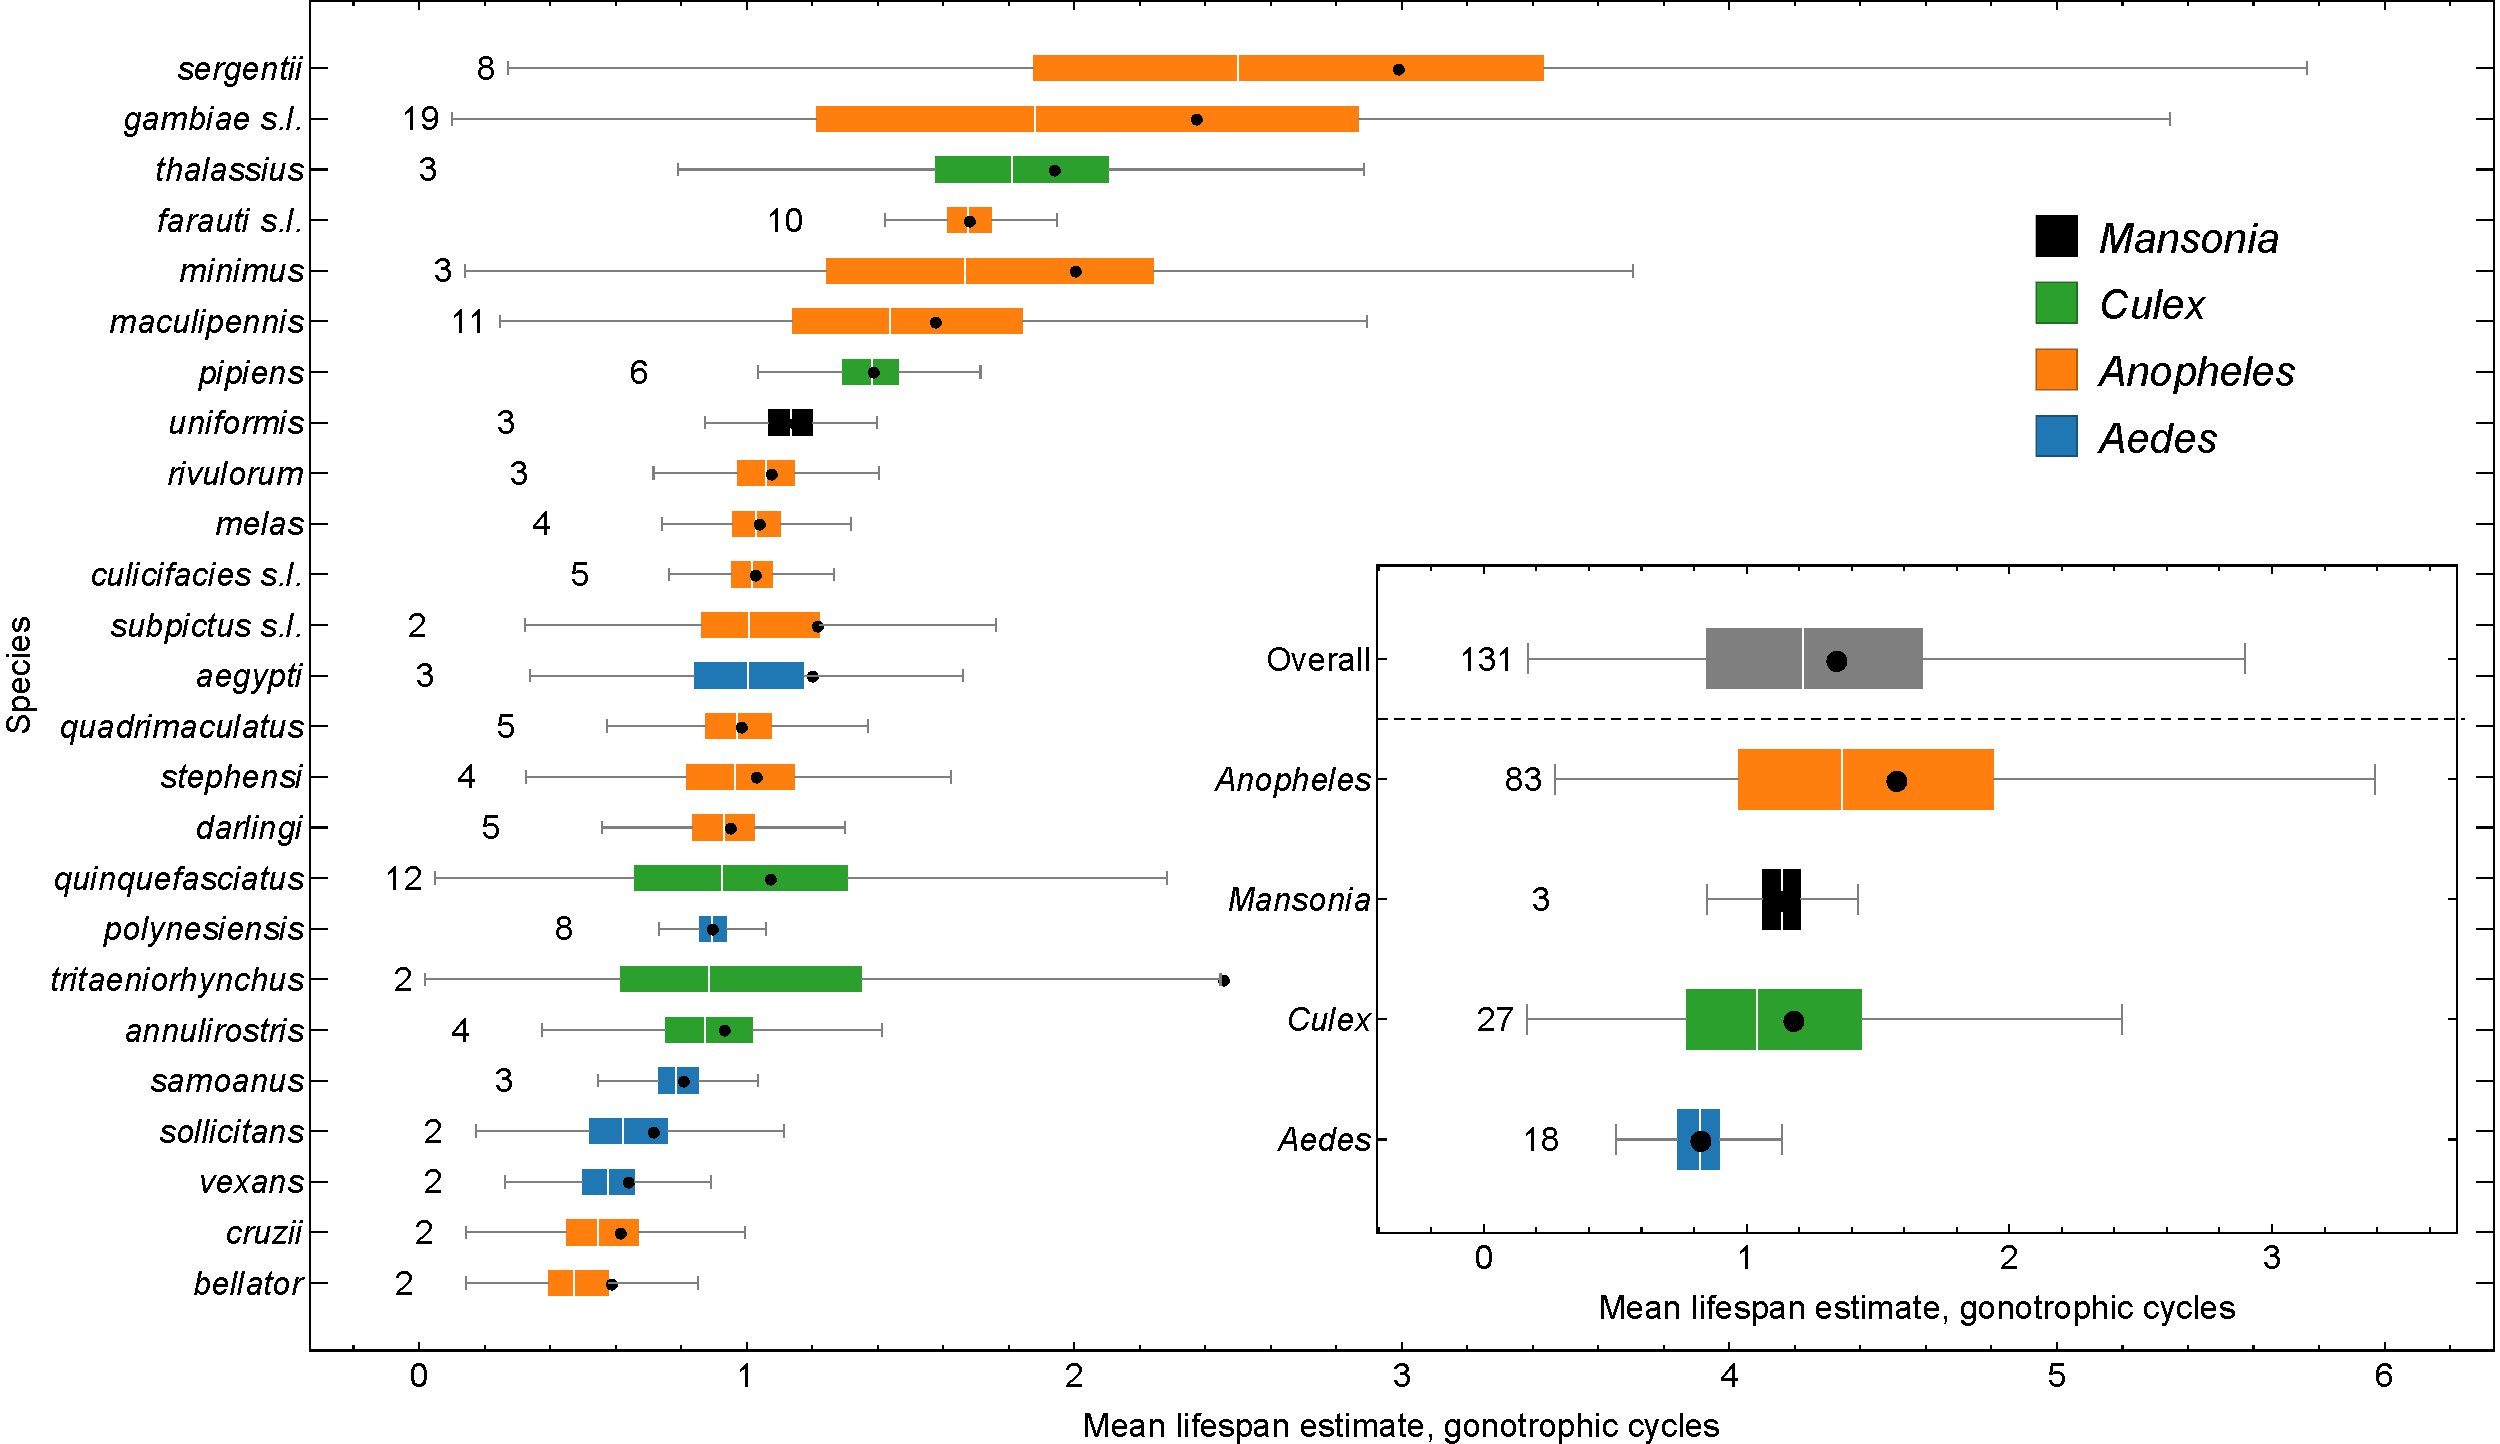
\includegraphics[width=1\textwidth]{./Figure_files/dissection_lifetimes_exponential.pdf}}
	\caption{\textbf{Polovodova dissection: grouped physiological lifespan estimates.} The lifespans shown are for mosquitoes that were not fed with sugar or blood (for females) before release. The middle line in each box shows the median estimates and the solid dot indicates the mean. The left and right box edges show the 25\%, and 75\% posterior quantiles respectively. The whiskers show the range of the data, excluding points lying more than 1.5 times the interquartile range away from each edge of the box. The numbers before the start of the left whisker indicate the number of individual time-series within each species. All estimates were obtained using the hierarchical exponential survival model.}
	\label{fig:dissection_lifetimes_exponential}
\end{figure}

\begin{figure}[h]
	\centerline{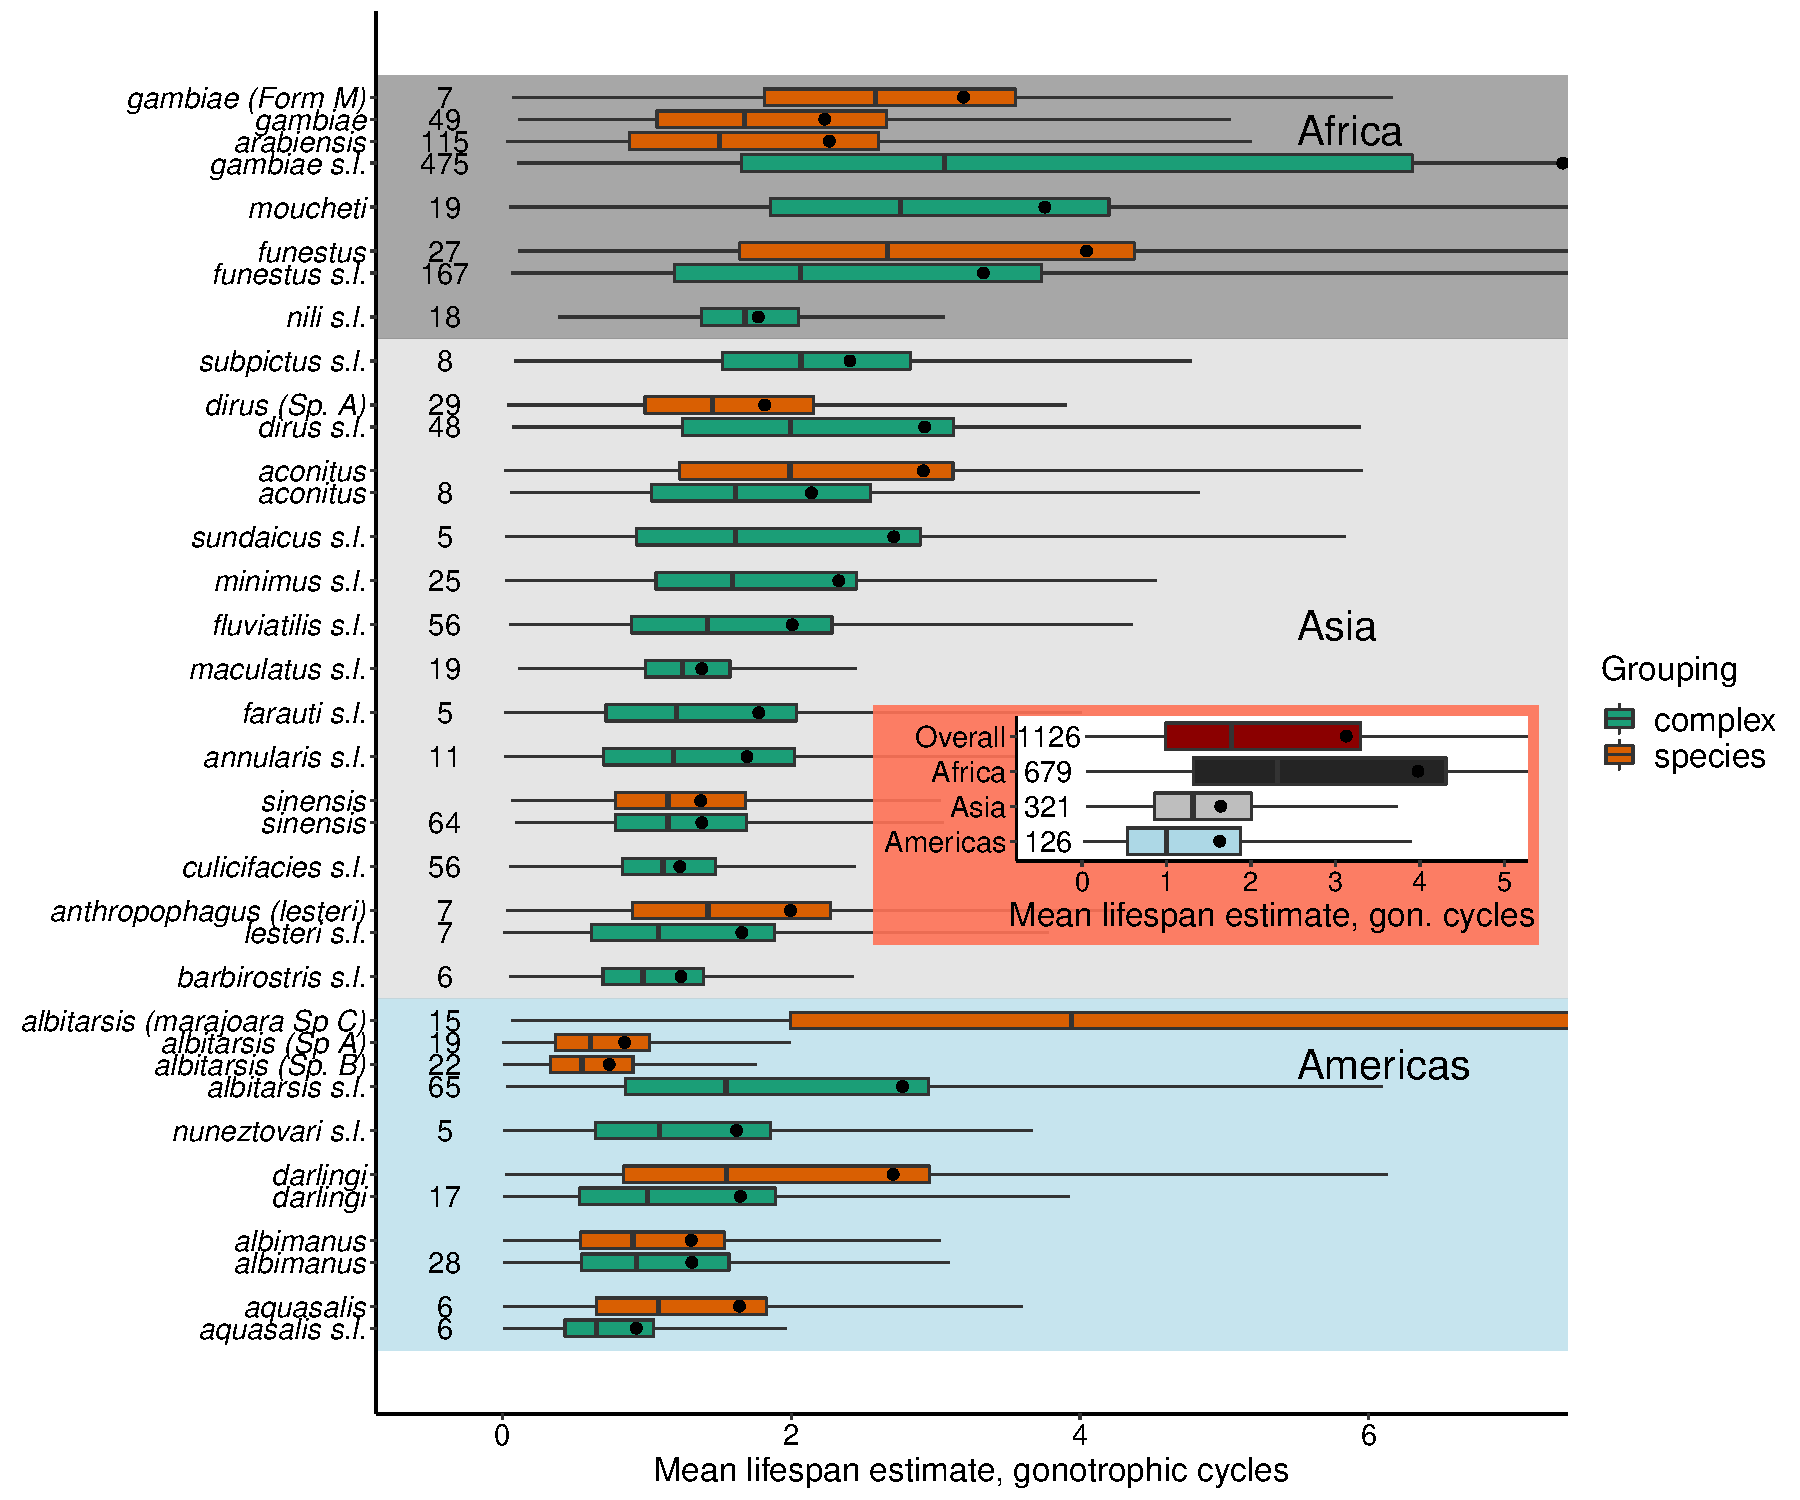
\includegraphics[width=1\textwidth]{./Figure_files/detinova_lifespans_combined_parity_no_insecticide.pdf}}
	\caption{\textbf{Detinova dissection: grouped lifespan estimates for anophelines.} As described in SOM, both species and morphospecies estimates are provided where available. The three coloured backgrounds show data according to continent where experiment was carried out (Americas-blue, Asia-grey, Africa-black). The middle line in each box shows the median estimates and the solid dot indicates the mean. The left and right box edges show the 25\%, and 75\% posterior quantiles respectively. The whiskers show the range of the data, excluding points lying more than 1.5 times the interquartile range away from each edge of the box. The numbers before the start of the left whisker indicate the number of individual time-series within each species.}
	\label{fig:detinova_lifetimes}
\end{figure}

\begin{figure}[h]
	\centerline{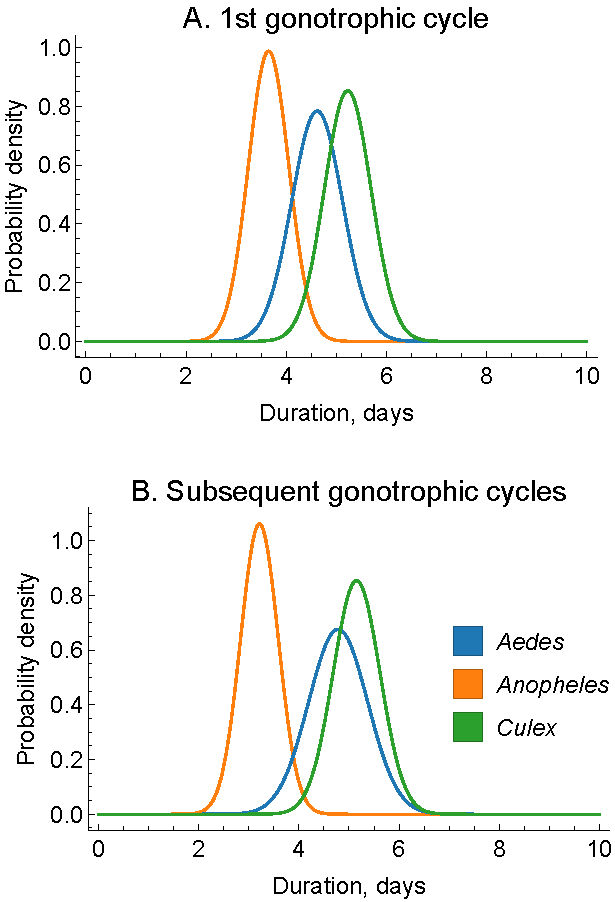
\includegraphics[width=0.7\textwidth]{./Figure_files/gonotrophic_cycle_durations.pdf}}
	\caption{\textbf{Estimates of gonotrophic cycle duration.} Coloured lines represent different genera, with each line indicating the estimated Gaussian probability density representing uncertainty over the reproductive cycle length.}
	\label{fig:gonotrophic}
\end{figure}

\begin{figure}[h]
	\centerline{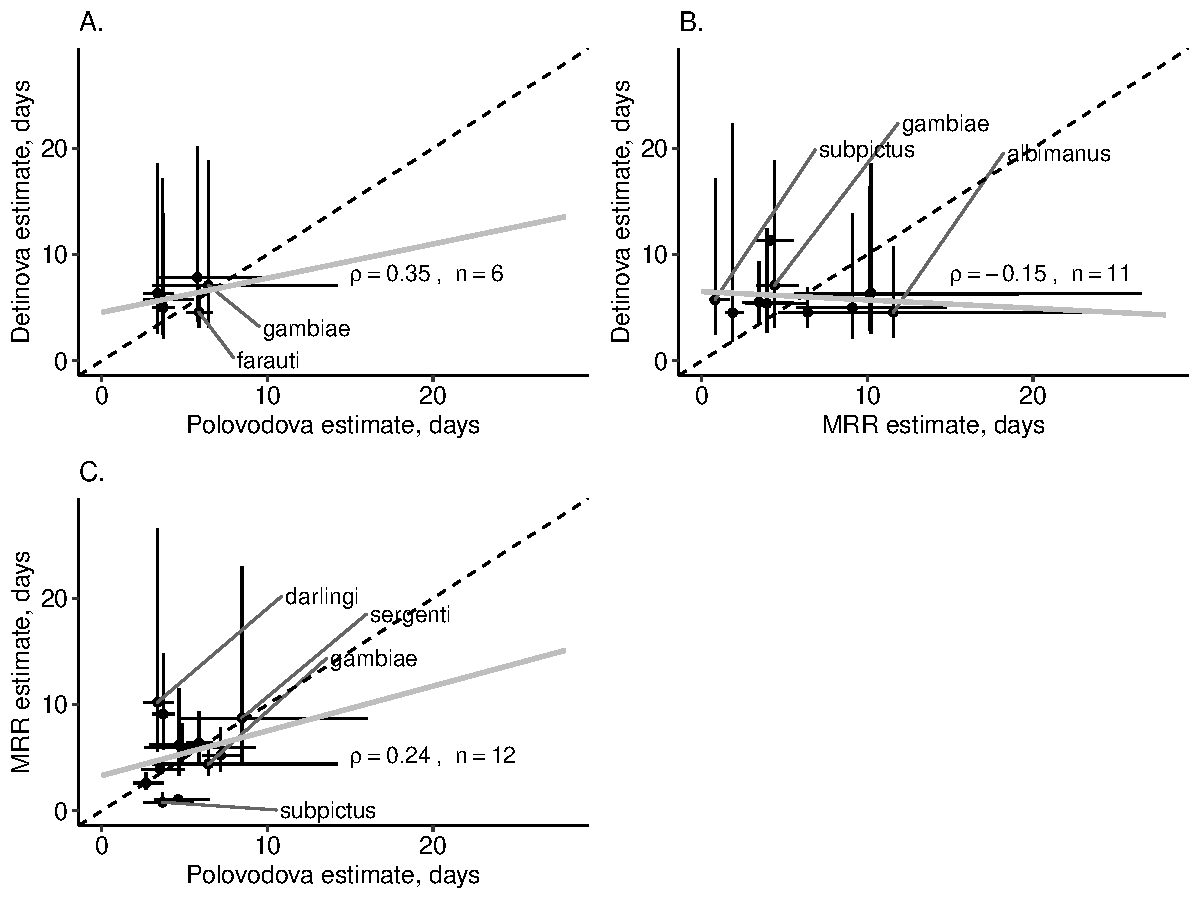
\includegraphics[width=1.3\textwidth]{./Figure_files/pairwise_comparison.pdf}}
	\caption{\textbf{Comparing lifespan estimates.} In A, B and C, we show pairwise estimates of lifespan for those species available in both datasets. For the MRR data, we show estimates for females that were neither fed with sugar or blood pre-release. Points indicate the posterior mean estimates and the whiskers show 25\% and 75\% quantiles. The values of $\rho$ indicate Pearson correlations (in no cases were these significant) and $n$ indicates sample size.}
	\label{fig:comparison}
\end{figure}

\begin{figure}[h]
	\centerline{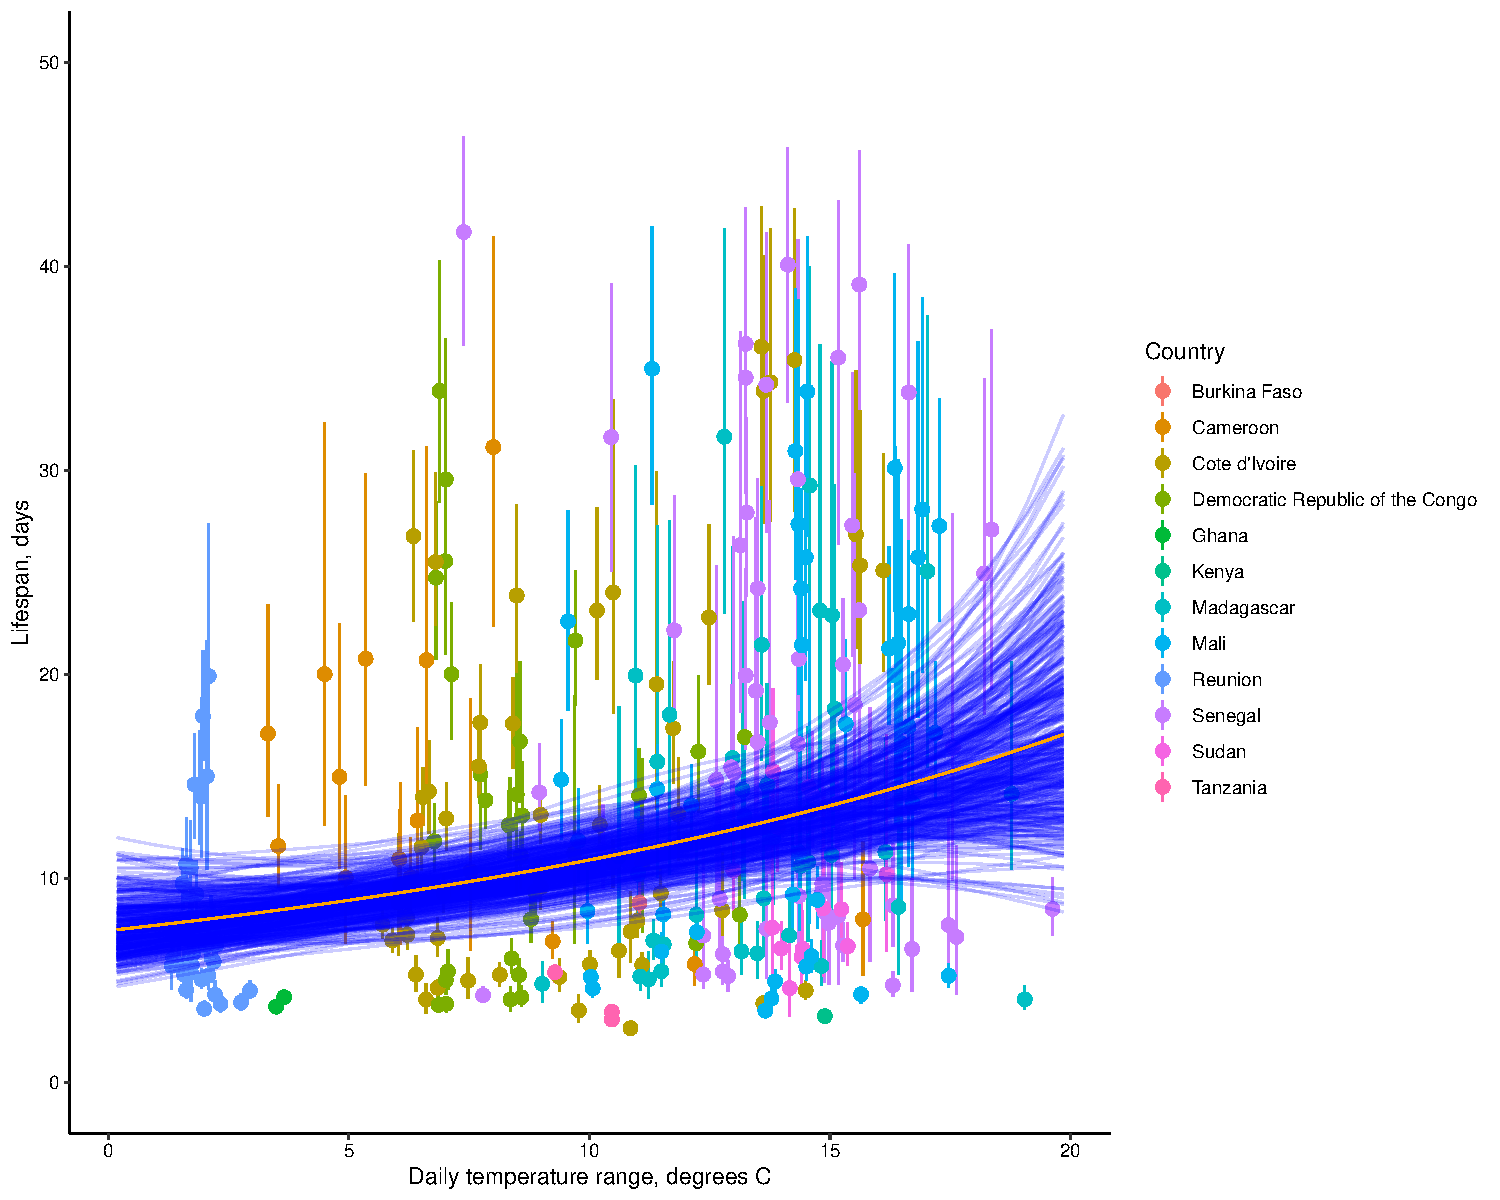
\includegraphics[width=1.3\textwidth]{./Figure_files/detinova_gambiae_daynight_range_lifespan_country.pdf}}
	\caption{\textbf{Detinova dissection: day-night temperature range versus lifespan estimates for \textit{Anopheles gambiae s.l.}.} Points indicate the posterior mean estimates and the whiskers show 25\% and 75\% quantiles. Each blue line indicates a posterior estimate of the relationship between lifespan and temperature range; the orange line indicates the posterior median.}
	\label{fig:detinova_gambiae_daynight_range_lifespan_country}
\end{figure}

\begin{figure}[h]
	\centerline{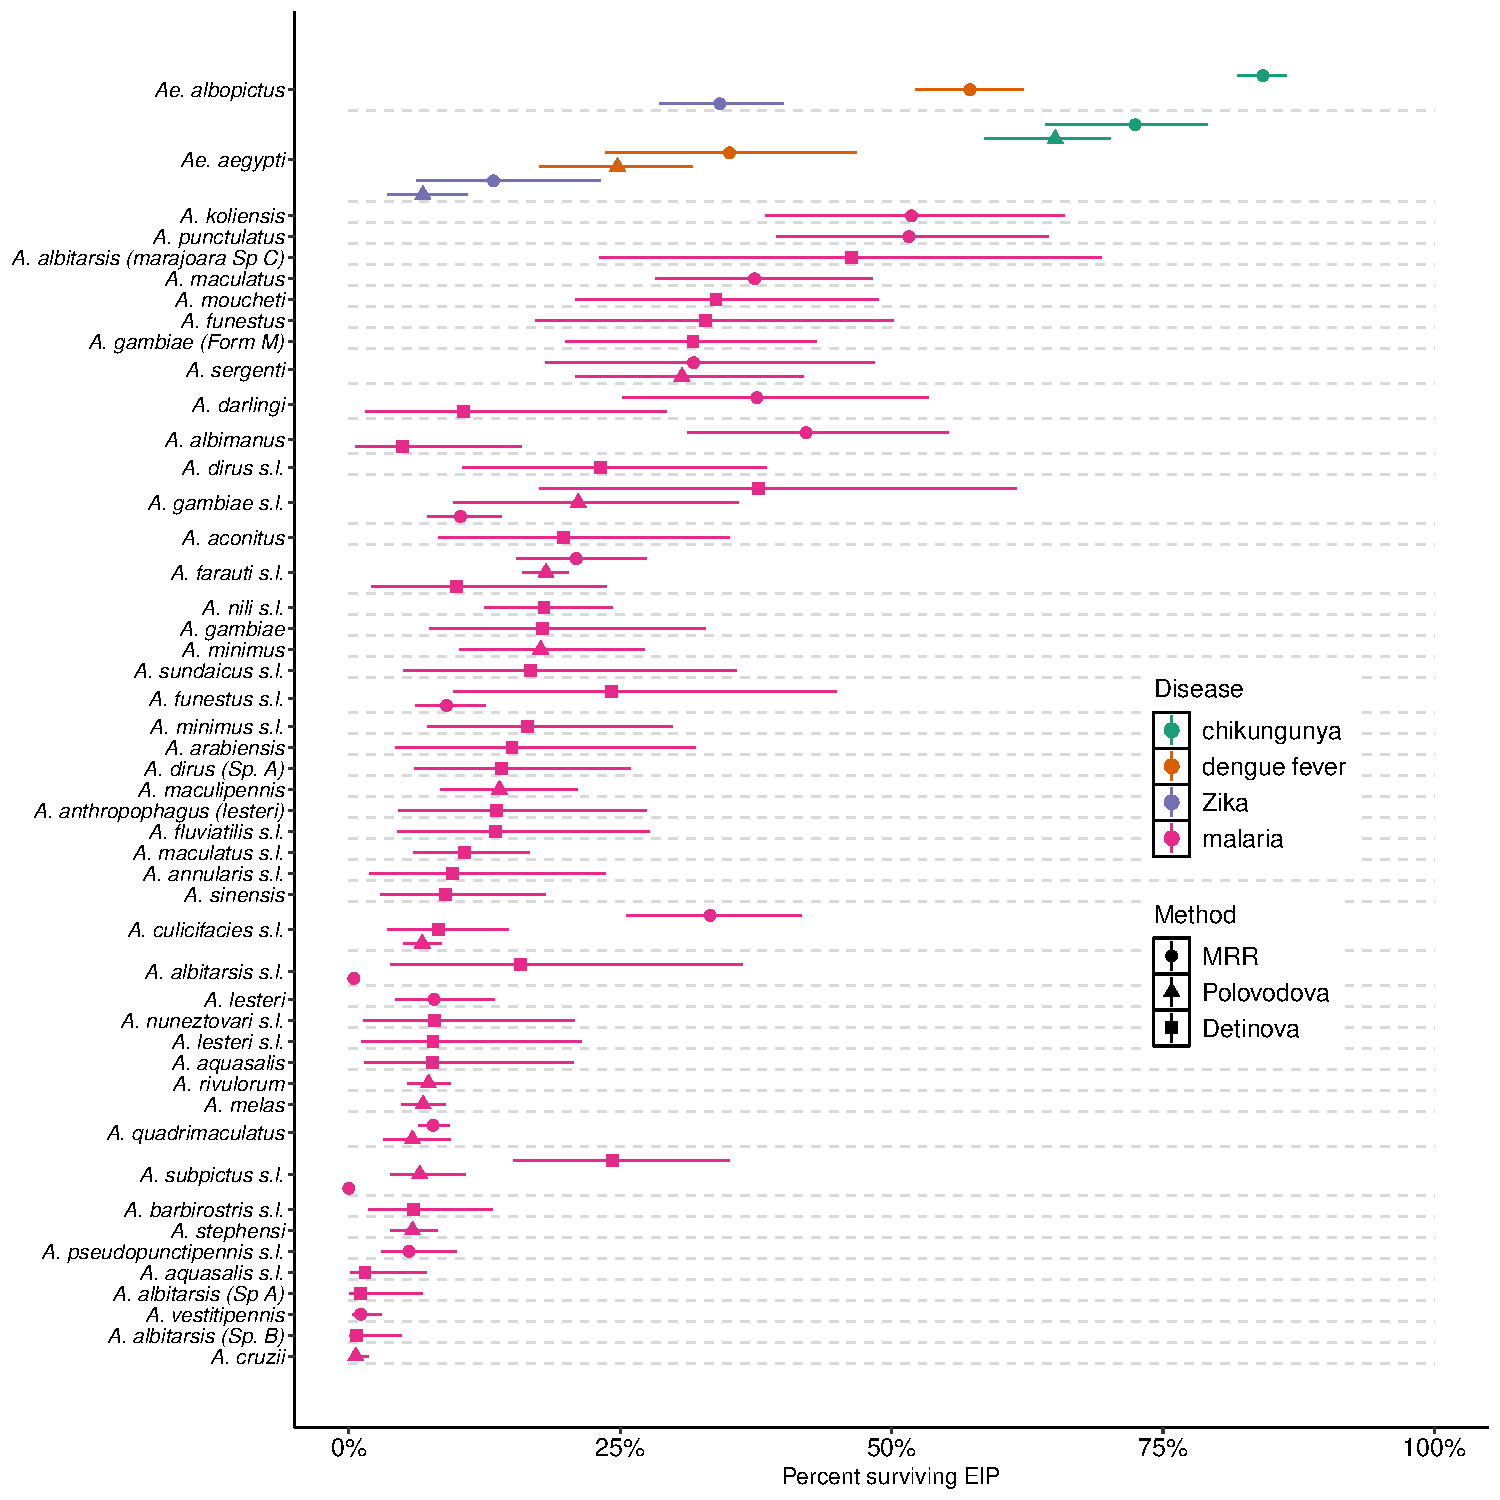
\includegraphics[width=1.3\textwidth]{./Figure_files/eip_all_combined.pdf}}
	\caption{\textbf{Proportions of mosquitoes surviving EIPs of malaria, dengue, chikungunya and Zika.} Colours indicate the measures for the different diseases; shapes indicate the dataset used to produce the estimate. We assumed that the EIPs were: malaria-10 days, chikungunya-2 days, dengue fever-6.5 days and Zika-12.5 days. The left and right whiskers indicate the 25\% and 75\% posterior quantiles, and the points indicate the mean. All estimates were obtained using the exponential survival model.}
	\label{fig:eip}
\end{figure}

\begin{figure}[h]
	\centerline{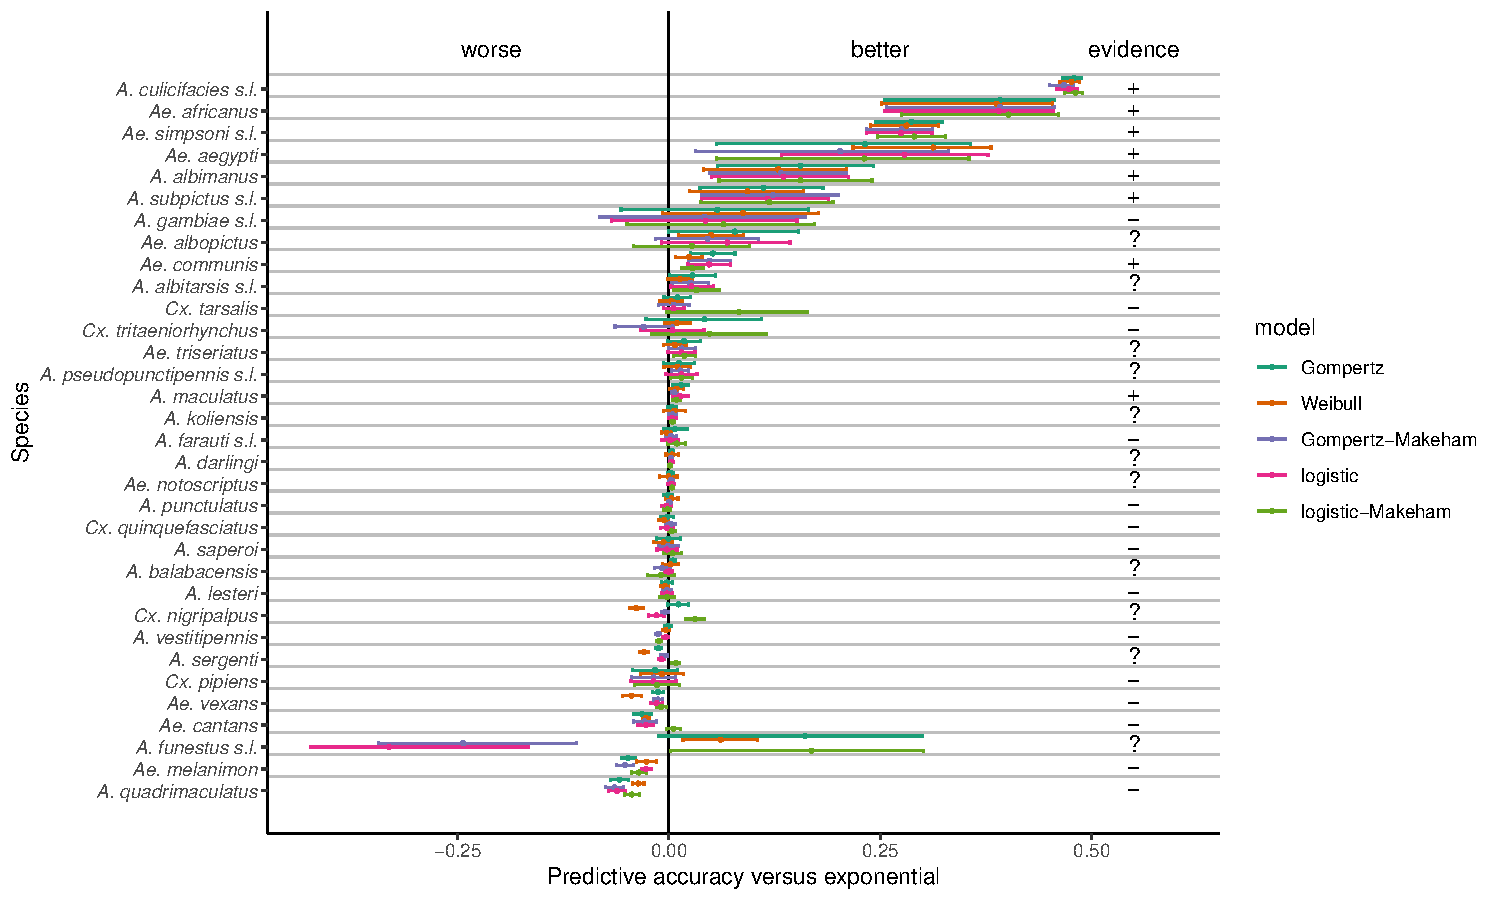
\includegraphics[width=1.3\textwidth]{./Figure_files/mrr_elpd_vs_exponential_ordered.pdf}}
	\caption{\textbf{MRR: evidence for senescence.} Here, we consider the predictive accuracy of age-dependent models of mortality versus the exponential model by species. The predictive accuracy was determined using K-Fold cross-validation as described in SOM; the measure of accuracy presented here by the central dots is the difference in estimated expected log pointwise predictive density compared to the exponential model. The lower and upper whiskers represent the lower and upper bounds of the 95\% confidence interval in predictive accuracy. The species have been ordered so that those with the highest average predictive accuracy across all age-dependent models compared to the exponential model appear at the top. If all age-dependent models outperform the exponential, we deem this as evidence for age-dependent mortality (`+'); if a subsample of models perform better, we deem the evidence ambiguous (`?'); and if no age-dependent model exceeds the performance of the exponential, we conclude no evidence in favour of senescence (`-').}
	\label{fig:mrr_elpd}
\end{figure}





\end{document}